\authoredSection{corny}{Toolchain}
Im Rahmen unseres Projekts wurde uns schnell klar, dass wir auf viele Tools angewiesen sein würden. So musste unser Quelltext versioniert, die grobe Struktur und Views festgehalten und Aufgabenpakete erstellt und koordiniert werden. Darüber hinaus waren uns auch Design und Qualität wichtig. Auf unsere Erfahrungen in diesem Zusammenhang gehen wir im folgenden Abschnitt ein.

\subsection{Agiles Vorgehen im Projekt}
	Da uns freundlicherweise von der C1 WPS GmbH die Möglichkeit gegeben wurde, eine Scrum-Zer\-ti\-fi\-zie\-rung zu erhalten, lag uns viel daran, den Scrum-Ansatz so gut es ging in unseren Projekt-Ablauf zu integrieren. Zudem war es im Rahmen der wöchentlichen Projektdiskussion Vorgabe, den Fortschritt anhand eines Scrum-Tools dokumentiren zu können.
	
	Dazu verwendeten wir – nach ersten Versuchen mit GitHub-Issues – die Software PivotalTracker. Während GitHub zwar eine für andere Zwecke ausreichende Möglichkeit bietet, sogenannte Issues anzulegen und abzuarbeiten, kann PivotalTracker den gesamten Scrum-Ablauf abbulden.
	Beispielsweise können wir, wie in Abbildung \ref{fig:TrackerStories} dargestellt, einzelne Stories erstellen und überwachen. Ein großer Vorteil dabei war, dass Scrum-Iterationen automatisch von der Software generiert werden, berechnet durch unsere durchschnittliche Arbeitskraft (genannt „Velocity“)\footnote{\url{http://www.pivotaltracker.com/community/tracker-blog/velocity-matters}} und unseren Vorhersagen für den Aufwand einer Story angegeben durch Punkte.
	
\begin{figure}[h!]
	\centering
	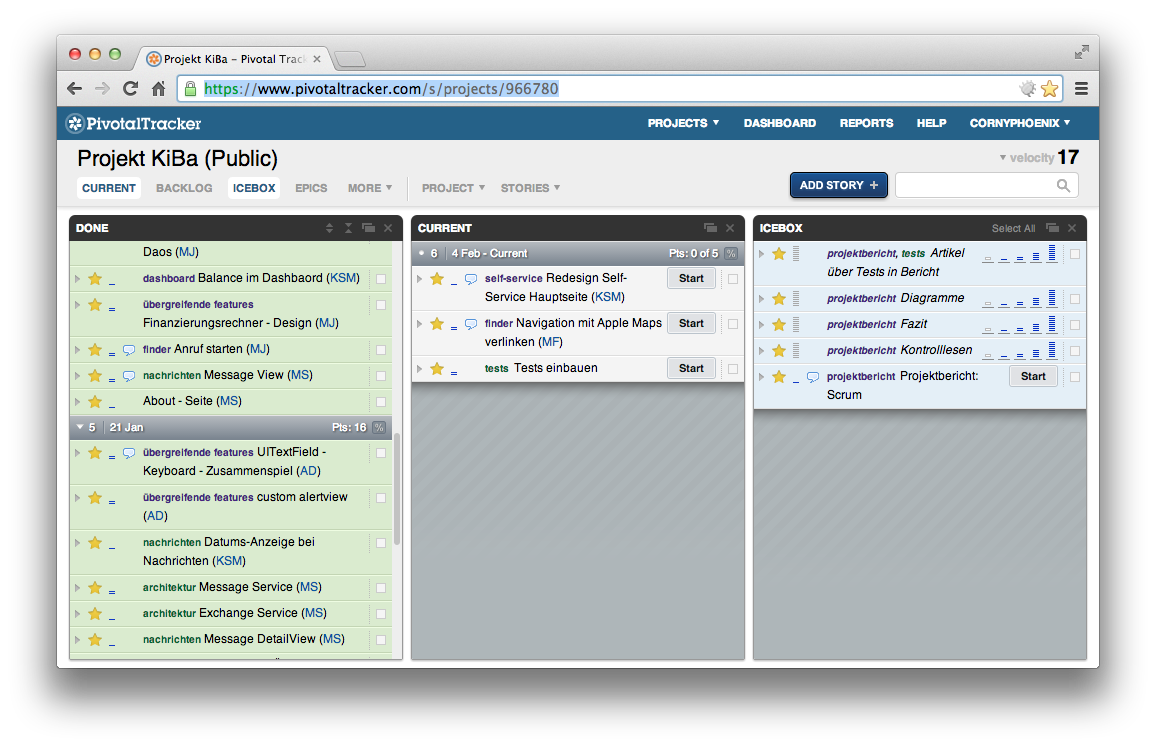
\includegraphics[scale=.25]{Pictures/TrackerStories}
	\vspace{-.8cm}
	\caption{Stories in PivotalTracker\label{fig:TrackerStories}}
\end{figure}

\noindent	Zum anderen generiert PivotalTracker auch Burndown-Charts, welche für das Vorgehen während der Scrum-Iterationen unabdinglich sind. Denn so können wir am besten den Fortschritt unserer App messen und haben ein Monitoring für das Fortschreiten der Entwicklung unserer Features, wie in Abbildung \ref{fig:TrackerBurndown} zu sehen ist.

\begin{figure}[h]
	\centering
	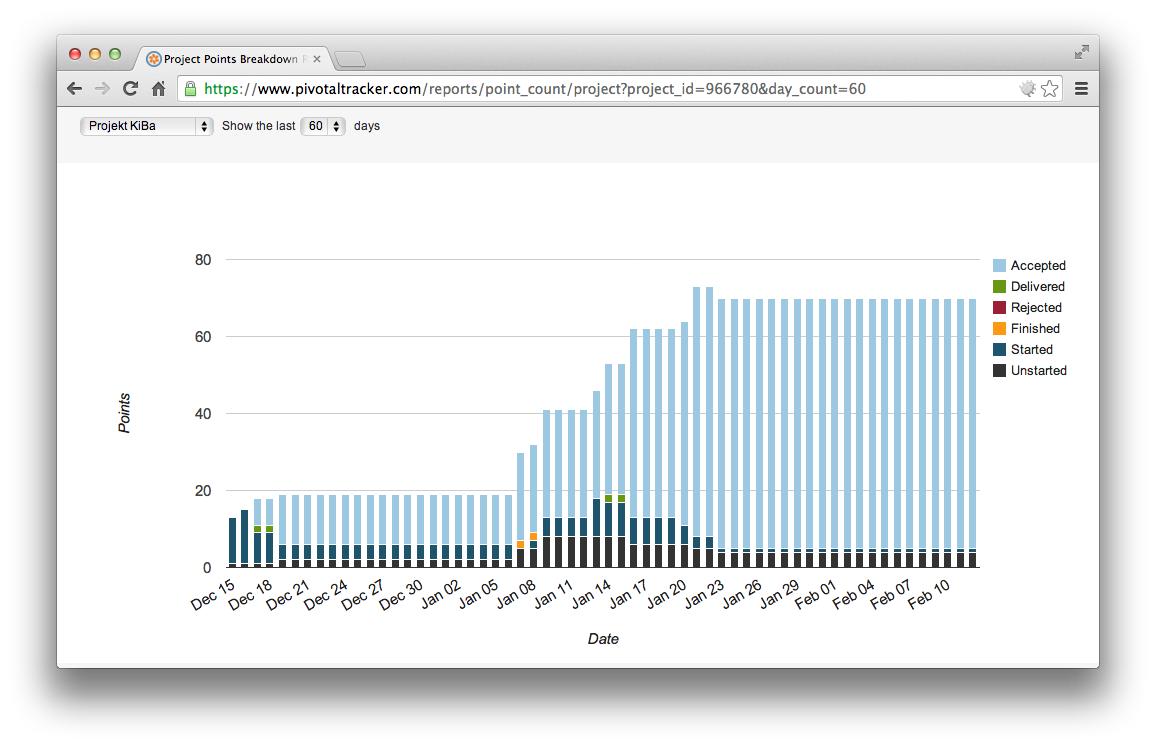
\includegraphics[scale=.25]{Pictures/TrackerBurndown}
	\vspace{-.8cm}
	\caption{Burndown-Chart in PivotalTracker\label{fig:TrackerBurndown}}
\end{figure}

\subsection{Versionsverwaltung und Informationsaustausch}
	Um kollaborativ an einer Software zu arbeiten, ist es selbstverständlich erforderlich, mit Quelltextversionierung zu arbeiten. Da bei uns Team-Mitgliedern die Erfahrung mit Git\footnote{\url{http://git-scm.com/}} aus dem Universitäts- und Arbeitsumfeld am größten war, fiel unsere Wahl für ein \acs{VCS} darauf. Entscheidend dabei war auch der größere Komfort gegenüber Subversion und die Möglichkeit, die Plattform GitHub\footnote{\url{https://github.com/}} als Repository-Hoster und anfangs auch als Issue-Tracker zu verwenden. Wie unser Repository bei GitHub aussieht, ist in Abbildung \ref{fig:GitHubOverview} zu sehen.
	
	Ein weiteres nützliches Feature von GitHub für uns war außerdem ein Wiki, dargestellt in Abbildung \ref{fig:GitHubWiki}. In ihm tauschen wir Informationen aus, wie beispielsweise erste Feature-Ideen oder Kontaktdaten aller Mitglieder. Allerdings nutzten wir es darüber hinaus auch für das Festlegen eines Arbeitsablaufs mit Xcode.
	
\begin{figure}
	\centering
	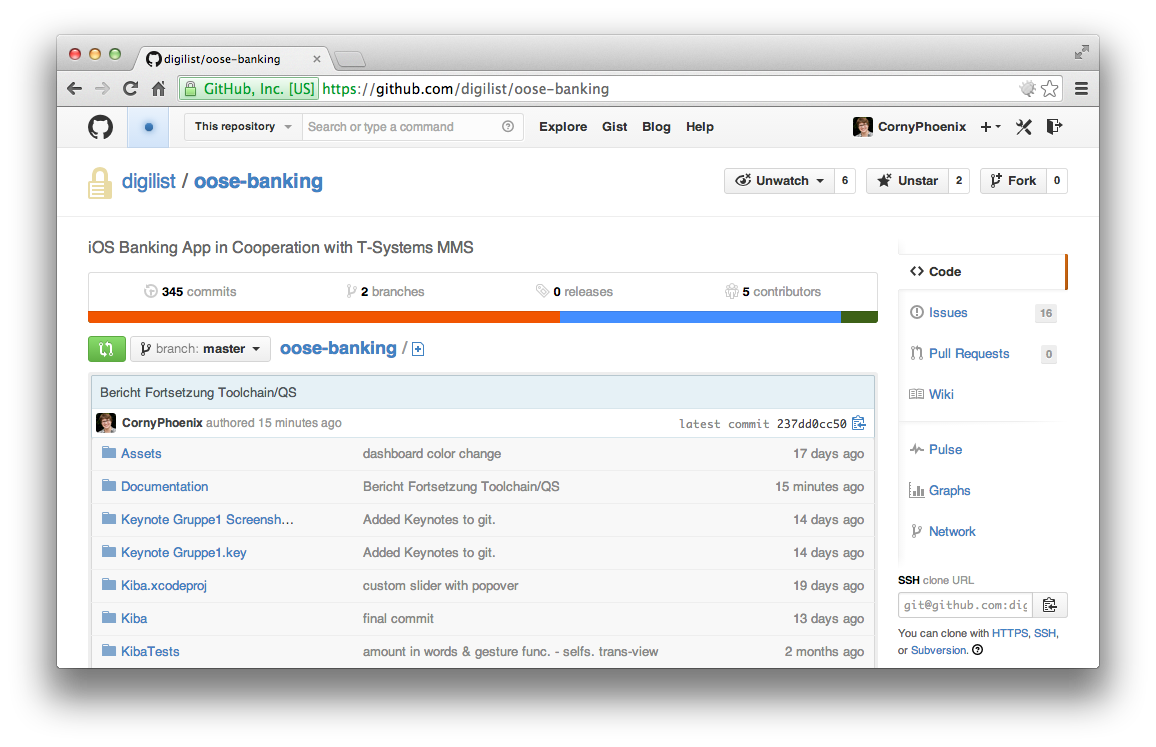
\includegraphics[scale=.25]{Pictures/GitHubOverview}
	\caption{Quelltext-Hosting bei GitHub \label{fig:GitHubOverview}}
\end{figure}

\begin{figure}
	\centering
	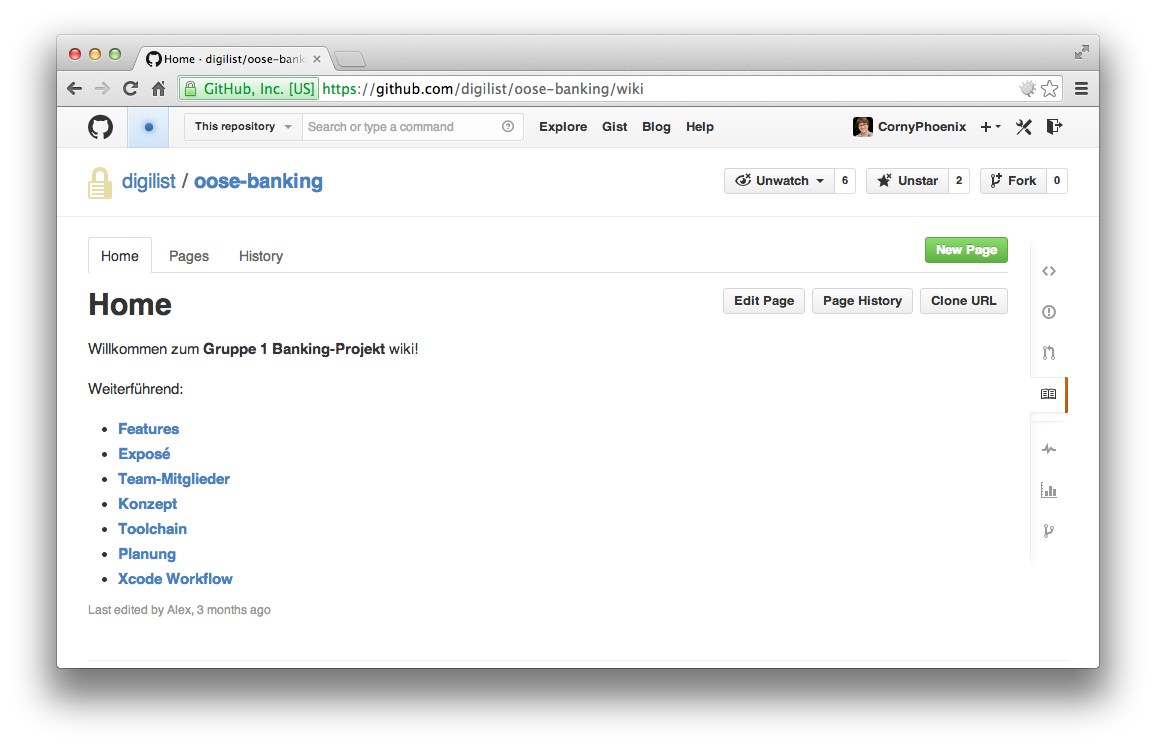
\includegraphics[scale=.25]{Pictures/GitHubWiki}
	\caption{GitHub-Wiki für den Wissensaustausch \label{fig:GitHubWiki}}
\end{figure}

\subsection{Konzept und erster Entwurf}
Balsamiq
\begin{figure}
	\centering
	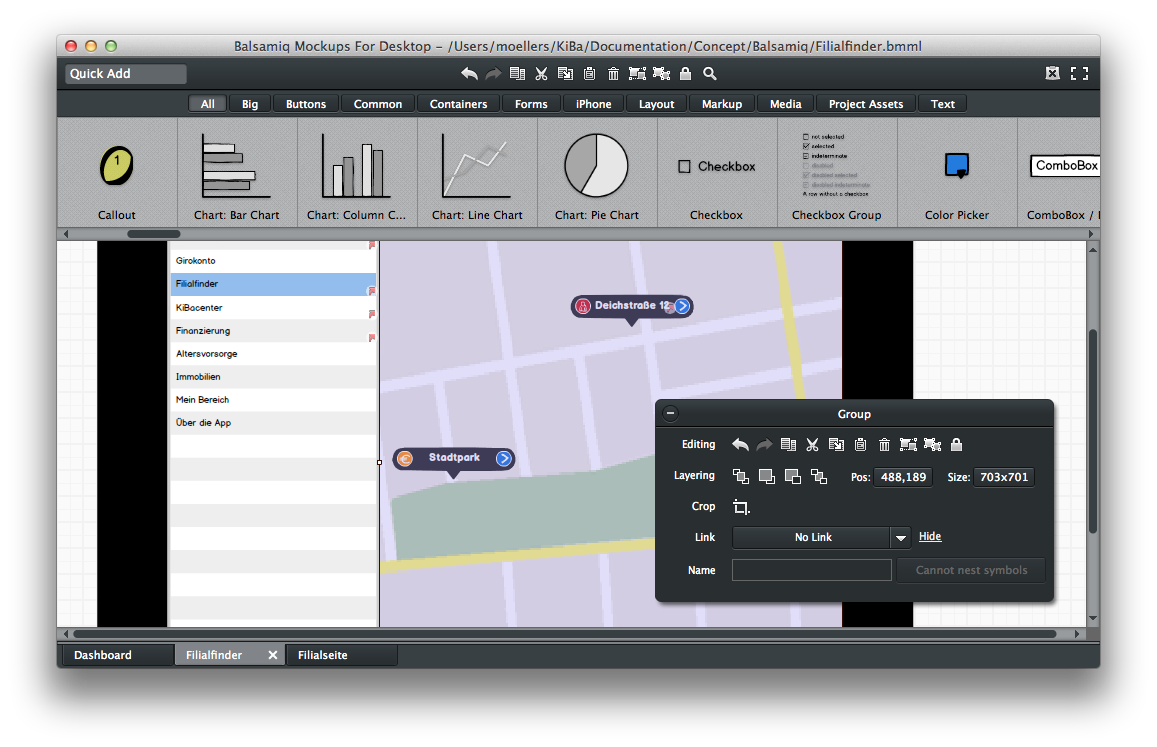
\includegraphics[scale=.3]{Pictures/BalsamiqEntwurf}
	\label{fig:BalsamiqEntwurf}
	\caption{Entwerfen mit Balsamiq}
\end{figure}

\subsection{Designtools}
Adobe Illustrator/Photoshop
\begin{figure}
	\centering
	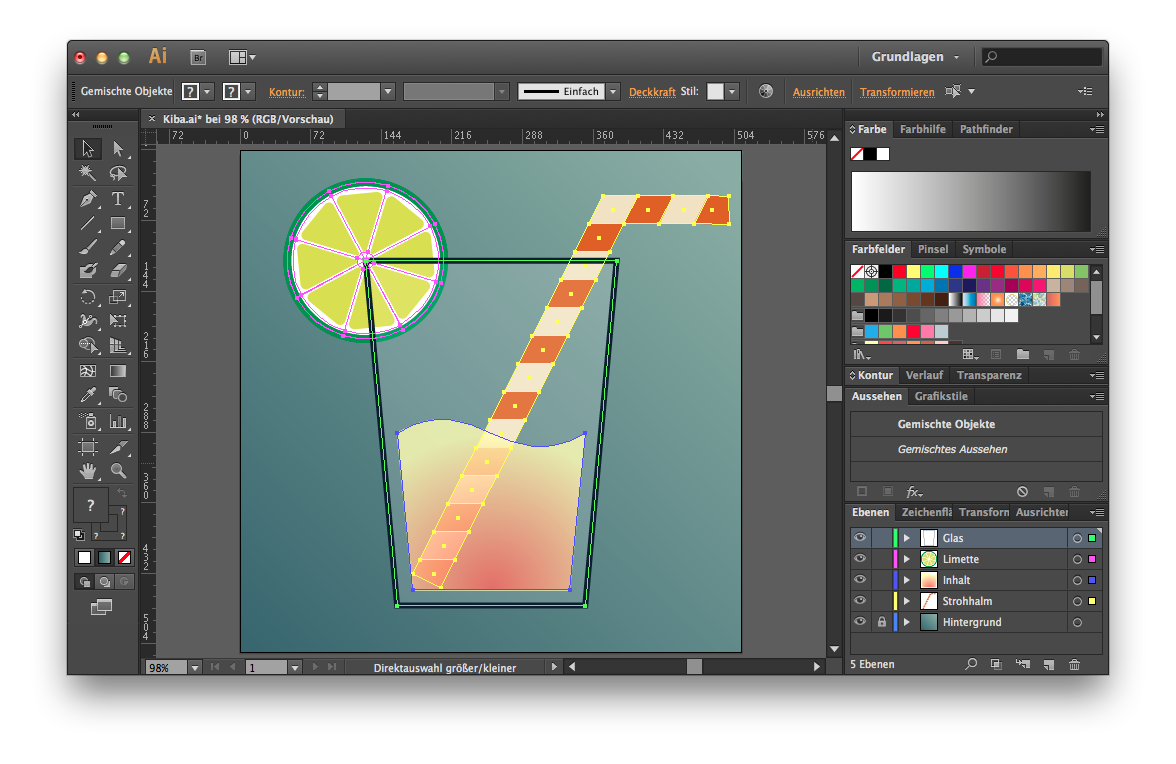
\includegraphics[scale=.3]{Pictures/IllustratorIcon}
	\label{fig:IllustratorIcon}
	\caption{Designen des KiBa-Icons mit Adobe Illustrator}
\end{figure}